\documentclass[10pt,openany,a4paper]{article}
\usepackage{tikz, pgfplots, tkz-euclide,calc}
\usetikzlibrary{patterns,shapes.arrows,calc}
\usepackage{fancyhdr}
\usepackage{enumerate,enumitem}
\usepackage{cancel}
\usepackage{varwidth}

% TAMBAHKAN PACKAGE SENDIRI KALAU KURANG

\usepackage{geometry}
\geometry{
	left = 22mm,
	right = 22mm,
	top = 25mm,
	bottom = 25mm,
}
\usepackage{graphicx}
\usepackage{subcaption}
\usepackage{soul}
\usepackage{hyperref}
\usepackage{float}
\usepackage{setspace}
\usepackage{afterpage}
\usepackage{xcolor}
\usepackage[nosectionbib]{apacite}
\usepackage{lmodern}
\usepackage{mathtools}
\usepackage{upgreek}
\usepackage{siunitx}
\usepackage{physics}
\usepackage{hyperref}
\renewcommand{\baselinestretch}{1.3}
\usepackage{multicol}
\usepackage{hyperref,ragged2e,amsmath,multicol,gensymb,setspace,
fancyhdr,amsfonts,tikz,pgfplots,nccmath,enumerate,verbatim,amsthm,physics}
\usepgfplotslibrary{polar,fillbetween}
% Enable tikz externalization; compile with -shell-escape when figures change
\usepgfplotslibrary{external}
\tikzexternalize[prefix=tikz/]
\tikzset{reuse path/.code={\pgfsyssoftpath@setcurrentpath{#1}}}
\tikzset{label kurva/.style={fill opacity=0, text opacity=1, inner sep=1.5pt, rounded corners=1pt}}
\usetikzlibrary{shapes.geometric,arrows}
\newcommand\mylog[1]{\mathop{{}^{#1}\mathrm{log}}}
\pgfplotsset{compat=1.15}
\pgfplotsset{my style/.append style={axis x line=middle, axis y line=
middle, xlabel={$x$}, ylabel={$y$}, axis equal }}
\usepackage{etoolbox}
% remove stray \makeatother
\newtheorem{defn}{Definisi}[section]
\newtheorem{teo}[defn]{Teorema}
\newtheorem{thm}{Teorema}[section]
\newtheorem{lemma}{Lemma}
\newtheorem{lemmas}[defn]{Lemma}
\newtheorem{cor}[defn]{Akibat}
\newtheorem{asumsi}[defn]{Asumsi}
\theoremstyle{definition}
\newtheorem{con}{Contoh}[section]
\theoremstyle{definition}
\theoremstyle{plain}
\newtheorem{prop}{Proposisi}[section]
\renewcommand{\proofname}{Bukti}
\renewcommand{\thethm}{\arabic{chapter}.\arabic{thm}}

\newcommand{\normlp}[1]{\left\|#1\right\|_{L^p_{\lambda}(0,T;H)}}% Fungsi norm (||x||)
\newcommand{\R}{\mathbb{R}}
\renewcommand{\natural}{\mathbb{N}}
\newcommand{\Xpl}{X^R_{p,\lambda}}
\newcommand{\Xpls}{X^R_{p,\lambda^*}}
\newcommand{\qpl}{q^R_{p,\lambda}}
\newcommand{\qpls}{q^R_{p,\lambda^*}}
\pagestyle{fancy}
\fancyhf{}
\lhead{Halaman \thepage}
\rhead{Pembahasan Soal ETS 2023/2024 \\ (\href{https://instagram.com/ahmadzakiyudin_/}{@ahmadzakiyudin\_})}
\hypersetup{
    colorlinks=true,
    linkcolor=blue,
    filecolor=blue,      
    urlcolor=blue,
}
\newenvironment{jawab}[2][tes]{
% \fbox{\begin{minipage}{14.65cm}
\textbf{Kata kunci materi:} #1.\\
\textbf{Penyelesaian:} #2
% \end{minipage}}
}{}

\newenvironment{jawab2}[2][tes]{
\fbox{\begin{minipage}{14.65cm}
 #2
\end{minipage}}}{}

\newenvironment{jawaban}[2][tes]{
\colorlet{oldcolor}{.}
        \color{red}
        \setlength{\fboxrule}{1pt}\boxed{\color{oldcolor}#2}\color{oldcolor}.
}{}

\newenvironment{jawaban2}[2][tes]{
\colorlet{oldcolor}{.}
        \color{red}
        \setlength{\fboxrule}{1pt}\fbox{\color{oldcolor}#2}\color{oldcolor}.
}{}

\newenvironment{penting}[2][tes]{
\colorlet{oldcolor}{.}
\color{blue}
\fbox{\color{oldcolor}#2}\color{oldcolor}
}{}

\begin{document}
\allowdisplaybreaks
\setlength\fboxsep{3pt}
% ensure enough header height for fancyhdr
\setlength{\headheight}{24pt}
\section*{Latihan Bab 5.4}
\begin{enumerate}
    \item Hitunglah luas daerah yang dibatasi oleh kurva $r=1+\sin \theta$ pada kuadran I.
            \begin{jawab}[luas daerah kurva polar, integral fungsi trigonometri]{
                \begin{center}
                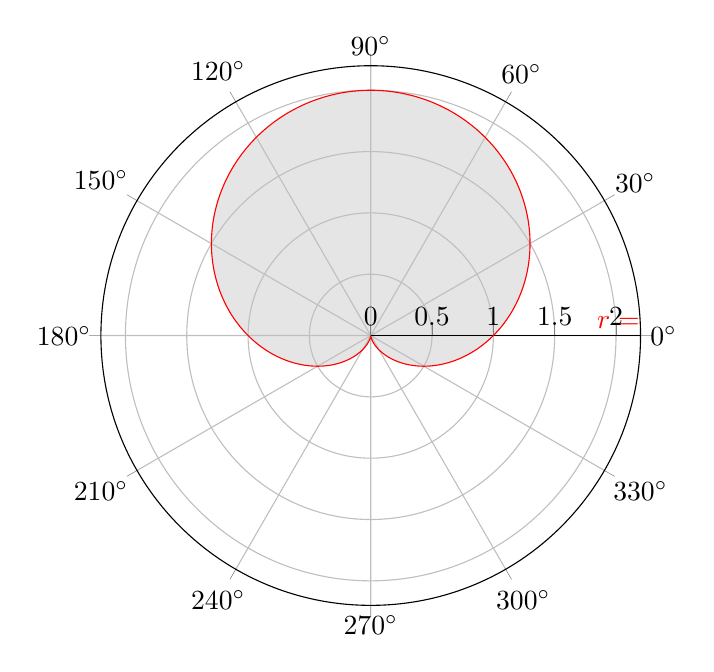
\begin{tikzpicture}
\pgfplotsset{set layers}
  \begin{polaraxis}[xticklabel={$ \pgfmathprintnumber{\tick}^{\circ} $}]
    \addplot[domain=0:360,samples=1000, color=red, save path=\kardioda] {1+sin(x)};
    \node[red,label kurva,anchor=south west] at (rel axis cs:0.14,0.82) {$r=1+\sin\theta$};
    \pgfonlayer{axis background}
    \fill[gray!20, reuse path=\kardioda];
    \endpgfonlayer
    \end{polaraxis}
                \end{tikzpicture}
            \end{center}
            Daerah yang diminta berada pada kuadran I, sehingga batas sudutnya adalah $\theta=0$ sampai $\theta=\frac{\pi}{2}$. Ingat kembali bahwa luas daerah yang dibatasi oleh kurva polar $r=f(\theta)$ dari $\theta=a$ hingga $\theta=b$ dapat dihitung menggunakan rumus
\begin{align*}
    \colorlet{oldcolor}{.}
        \color{blue}
        \setlength{\fboxrule}{1pt} \boxed{\color{oldcolor}A=\frac{1}{2}\int_a^b f(\theta)^2\,d\theta}\color{oldcolor}.
\end{align*}
            \allowdisplaybreaks
            \begin{align*}
                L &= \int_0^{\pi/2} \frac{1}{2}(1+\sin \theta)^2 \, d\theta\\
                &= \frac{1}{2} \int_0^{\pi/2} (1 + 2\sin \theta + \sin^2 \theta) \, d\theta\\
                &= \frac{1}{2} \int_0^{\pi/2} \left(1 + 2\sin \theta + \frac{1 - \cos(2\theta)}{2}\right) \, d\theta\\
                &= \frac{1}{2} \int_0^{\pi/2} \left(\frac{3}{2} + 2\sin \theta - \frac{\cos(2\theta)}{2}\right) \, d\theta\\
                &= \frac{1}{2} \left[\frac{3}{2}\theta - 2\cos \theta - \frac{\sin(2\theta)}{4}\right]_0^{\pi/2}\\
                &= \frac{1}{2} \left[\frac{3\pi}{4} - 2\cdot 0 - \frac{\sin(\pi)}{4} - \left(0 - 2\cdot 1 - \frac{\sin(0)}{4}\right)\right]\\
                &= \frac{1}{2} \left[\frac{3\pi}{4} + 2\right]\\
                &= \begin{jawaban}{\frac{3\pi}{8} + 1}\end{jawaban}
            \end{align*}
            }
            \end{jawab}
            \item Hitunglah luas daerah yang dibatasi oleh kurva $r=2+2\cos \theta$.
            \begin{jawab}[luas daerah kurva polar, integral fungsi trigonometri]{
            %Kardioda $r=2+2\cos\theta$
            \begin{center}
                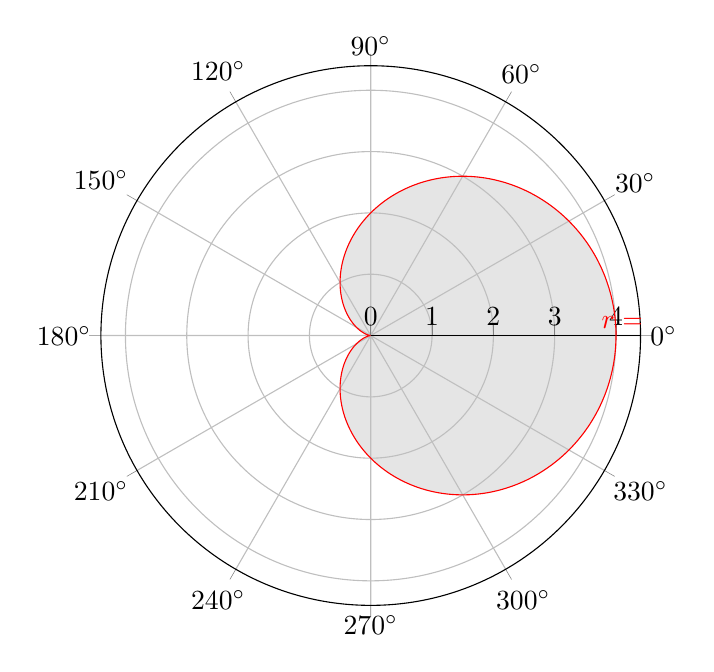
\begin{tikzpicture}
\pgfplotsset{set layers}
  \begin{polaraxis}[xticklabel={$ \pgfmathprintnumber{\tick}^{\circ} $}]
    \addplot[domain=0:360,samples=1000, color=red, save path=\kardioda] {2+2*cos(x)};
    \node[red,label kurva,anchor=south west] at (rel axis cs:0.56,0.83) {$r=2+2\cos\theta$};
    \pgfonlayer{axis background}
    \fill[gray!20, reuse path=\kardioda];
    \endpgfonlayer
    \end{polaraxis}
                \end{tikzpicture}
            \end{center}
            Diperhatikan bahwa kurva tersebut \textbf{simetri} terhadap sumbu-$x$, sehingga kita dapat menghitung luas daerah di atas sumbu-$x$ lalu mengalikannya dengan 2. Daerah di atas sumbu-$x$ dibatasi oleh kurva untuk $\theta$ dari $0$ hingga $\pi$. Dengan demikian, didapatkan:
            \begin{align*}
                L &= 2\int_0^{\pi} \frac{1}{2}(2+2\cos \theta)^2 \, d\theta\\
                &= 2\frac{1}{2} \int_0^{\pi} 4(1+\cos \theta)^2 \, d\theta\\
                &= 4 \int_0^{\pi} (1 + 2\cos \theta + \cos^2 \theta) \, d\theta\\
                &= 4 \int_0^{\pi} \left(1 + 2\cos \theta + \frac{1 + \cos(2\theta)}{2}\right) \, d\theta\\
                &= 4 \int_0^{\pi} \left(\frac{3}{2} + 2\cos \theta + \frac{\cos(2\theta)}{2}\right) \, d\theta\\
                &= 4 \left[\frac{3}{2}\theta + 2\sin \theta + \frac{\sin(2\theta)}{4}\right]_0^{\pi}\\
                &= \begin{jawaban}{6\pi}\end{jawaban}
            \end{align*}
            }
            \end{jawab}
            \item Hitunglah luas daerah di luar kardioda $r=2-2\cos\theta$ dan di dalam lingkaran $r=4$.\\
            \begin{jawab}[luas kurva polar]{
                Untuk menghitung luas daerah yang dibatasi oleh dua kurva polar, kita perlu mencari titik potong antara kedua kurva tersebut. Titik potong terjadi ketika $r$ dari kedua kurva sama, yaitu:
\begin{align*}
2 - 2\cos \theta &= 4\\
-2\cos \theta &= 2\\
\cos \theta &= -1\\
\theta &= \pi
\end{align*}
Berikut adalah gambar dari kedua kurva tersebut:
            \begin{center}
                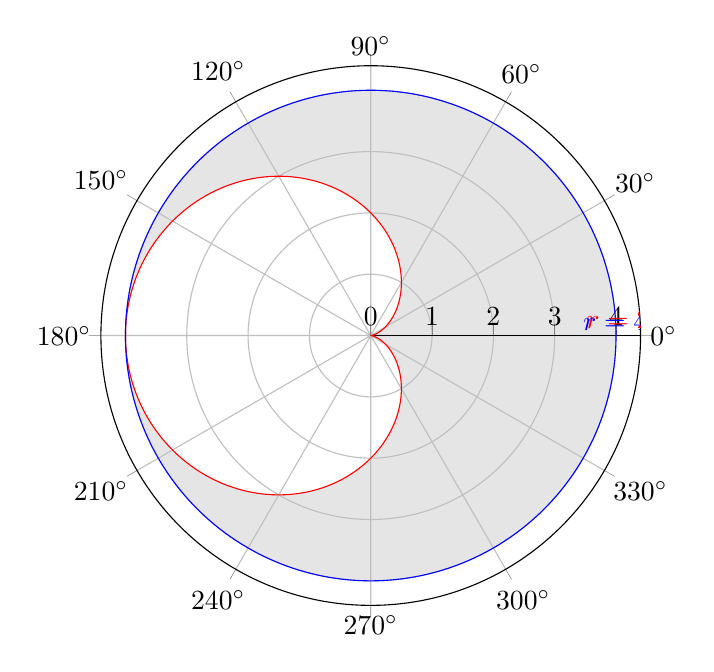
\begin{tikzpicture}
\pgfplotsset{set layers}
  \begin{polaraxis}[xticklabel={$ \pgfmathprintnumber{\tick}^{\circ} $}]
    \addplot[domain=0:360,samples=1000, draw=none, fill=gray!20, on layer=axis background] {4} \closedcycle;
    \addplot[domain=0:360,samples=1000, draw=none, fill=white, on layer=axis background] {2-2*cos(x)} \closedcycle;
    \addplot[domain=0:360,samples=1000, color=red] {2-2*cos(x)};
    \addplot[domain=0:360,samples=1000, color=blue] {4};
    \node[red,label kurva,anchor=south west] at (rel axis cs:0.16,0.78) {$r=2-2\cos\theta$};
    \node[blue,label kurva,anchor=south west] at (rel axis cs:0.77,0.76) {$r=4$};
    \end{polaraxis}
                \end{tikzpicture}
            \end{center}
            Ingat kembali bahwa luas daerah yang dibatasi oleh kurva polar $r=f(\theta)$ dari $\theta=a$ hingga $\theta=b$ dapat dihitung menggunakan rumus
\begin{align*}
    \colorlet{oldcolor}{.}
        \color{blue}
        \setlength{\fboxrule}{1pt} \boxed{\color{oldcolor}A=\frac{1}{2}\int_a^b f(\theta)^2\,d\theta}\color{oldcolor}.
\end{align*}
            Luas daerah yang dibatasi oleh kedua kurva tersebut adalah luas daerah di dalam lingkaran $r=4$ dikurangi dengan luas daerah di dalam kardioda $r=2-2\cos\theta$. Jelas bahwa luas lingkaran adalah $L=\pi r^2 = 16\pi$. Selanjutnya, kita hitung luas kardioda dengan menggunakan rumus luas kurva polar:
            \begin{align*}
L &= \int_0^{2\pi} \frac{1}{2}(2-2\cos \theta)^2 \, d\theta\\
&= \frac{1}{2} \int_0^{2\pi} 4(1-\cos \theta)^2 \, d\theta\\
&= 2 \int_0^{2\pi} (1 - 2\cos \theta + \cos^2 \theta) \, d\theta\\
&= 2 \int_0^{2\pi} \left(1 - 2\cos \theta + \frac{1 + \cos(2\theta)}{2}\right) \, d\theta\\
&= 2 \int_0^{2\pi} \left(\frac{3}{2} - 2\cos \theta + \frac{\cos(2\theta)}{2}\right) \, d\theta\\
&= 2 \left[\frac{3}{2}\theta - 2\sin \theta + \frac{\sin(2\theta)}{4}\right]_0^{2\pi}\\
&= 6\pi.
            \end{align*}
            Jadi luas daerah yang dibatasi oleh kedua kurva tersebut adalah:
            \begin{align*}
L &= 16\pi - 6\pi=\begin{jawaban}{10\pi}\end{jawaban}
                \end{align*}
            }
            \end{jawab}
            \item Hitung luas daerah di dalam lingkaran $r=5\sin\theta$ dan di luar limacon $r=2+\sin\theta$.\\
            \begin{jawab}[luas kurva polar]{
                Untuk menghitung luas daerah yang dibatasi oleh dua kurva polar, kita perlu mencari titik potong antara kedua kurva tersebut. Titik potong terjadi ketika $r$ dari kedua kurva sama, yaitu:
\begin{align*}
5\sin \theta &= 2 + \sin \theta\\
4\sin \theta &= 2\\
\sin \theta &= \frac{1}{2}\\
\theta &= \frac{\pi}{6}, \frac{5\pi}{6}
\end{align*}
Berikut adalah gambar dari kedua kurva tersebut:
            \begin{center}
                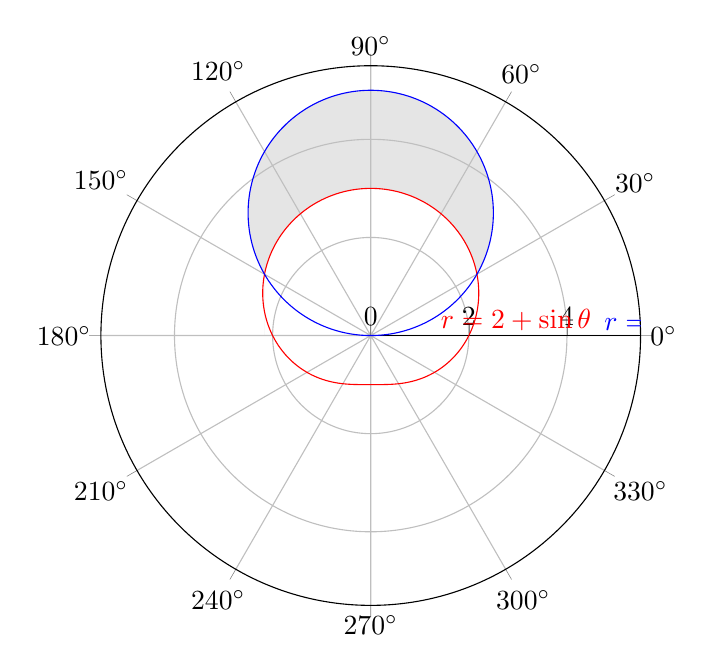
\begin{tikzpicture}
\pgfplotsset{set layers}
  \begin{polaraxis}[xticklabel={$ \pgfmathprintnumber{\tick}^{\circ} $}]
    \addplot[domain=30:150,samples=600, draw=none, fill=gray!20, on layer=axis background] {5*sin(x)} \closedcycle;
    \addplot[domain=30:150,samples=600, draw=none, fill=white, on layer=axis background] {2+sin(x)} \closedcycle;
    \addplot[domain=0:360,samples=1000, color=red] {2+sin(x)};
    \addplot[domain=0:360,samples=1000, color=blue] {5*sin(x)};
    \node[red,label kurva,anchor=south west] at (rel axis cs:0.67,0.24) {$r=2+\sin\theta$};
    \node[blue,label kurva,anchor=south west] at (rel axis cs:0.60,0.84) {$r=5\sin\theta$};
    \end{polaraxis}
                \end{tikzpicture}
            \end{center}
            Diperhatikan bahwa daerah tersebut \textbf{simetri} terhadap sumbu-$y$. Daerah yang diminta adalah luas daerah di dalam lingkaran $r=5\sin\theta$ pada interval $\left[\frac{\pi}{6},\frac{5\pi}{6}\right]$ dikurangi luas daerah di dalam limacon $r=2+\sin\theta$ pada interval yang sama. Dengan simetri, cukup dihitung bagian $\theta$ dari $\frac{\pi}{6}$ hingga $\frac{\pi}{2}$ lalu dikalikan 2.
            Didapatkan luasnya adalah 
            \begin{align*}
L &= 2\int_{\pi/6}^{\pi/2} \frac{1}{2}(5\sin \theta)^2 \, d\theta - 2\int_{\pi/6}^{\pi/2} \frac{1}{2}(2+\sin \theta)^2 \, d\theta\\
&= 2\int_{\pi/6}^{\pi/2} \frac{25}{2}\sin^2 \theta \, d\theta - 2\int_{\pi/6}^{\pi/2} \frac{1}{2}(4 + 4\sin \theta + \sin^2 \theta) \, d\theta\\
&= \int_{\pi/6}^{\pi/2} 25\sin^2 \theta-  (4+4\sin\theta+\sin^2\theta) \, d\theta \\
&= \int_{\pi/6}^{\pi/2} 24\sin^2\theta -4\sin\theta-4 \, d\theta\\
&= \int_{\pi/6}^{\pi/2} 24\qty(\frac{1-\cos (2\theta)}{2}) -4\sin\theta-4 \, d\theta\\
&= \int_{\pi/6}^{\pi/2} 12 - 12\cos (2\theta) -4\sin\theta-4 \, d\theta\\
&= \int_{\pi/6}^{\pi/2} 8 - 12\cos (2\theta) -4\sin\theta \, d\theta\\
&= \left[8\theta - 6\sin (2\theta) + 4\cos\theta\right]_{\pi/6}^{\pi/2}\\
&= \left(8\cdot \frac{\pi}{2} - 6\sin (\pi) + 4\cos\frac{\pi}{2}\right) - \left(8\cdot \frac{\pi}{6} - 6\sin \frac{\pi}{3} + 4\cos\frac{\pi}{6}\right)\\
&= 4\pi - \frac{4\pi}{3} + 6\cdot \frac{\sqrt{3}}{2} - 4\cdot \frac{\sqrt{3}}{2}\\
&= \begin{jawaban}{\frac{8\pi}{3} + \sqrt{3}}\end{jawaban}
\end{align*}
            }
            \end{jawab}
            \item Hitunglah luas daerah irisan dari lingkaran $r=3\cos\theta$ dan kardioda $r=1+\cos\theta$.
            \begin{jawab}[luas daerah]{
                Untuk menghitung luas daerah irisan dari dua kurva polar, kita perlu mencari titik potong antara kedua kurva tersebut. Titik potong terjadi ketika $r$ dari kedua kurva sama, yaitu:
\begin{align*}
3\cos \theta &= 1 + \cos \theta\\
2\cos \theta &= 1\\
\cos \theta &= \frac{1}{2}\\
\theta &= \frac{\pi}{3}, -\frac{\pi}{3}
\end{align*}
Jadi, titik potong antara kedua kurva tersebut terjadi pada \begin{penting}[]{$\theta=\frac{\pi}{3}$}\end{penting} dan \begin{penting}[]{$\theta=-\frac{\pi}{3}$}\end{penting}. Berikut adalah gambar dari kedua kurva tersebut:
            \begin{center}
                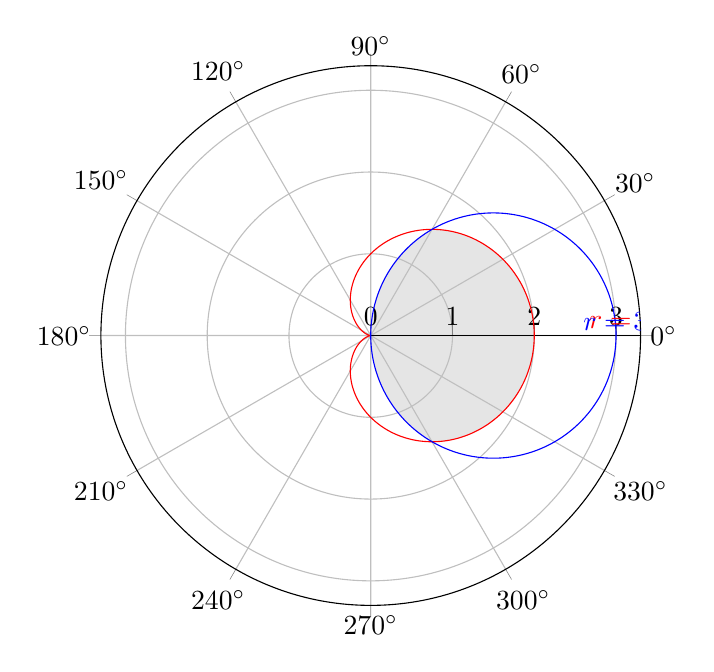
\begin{tikzpicture}
\pgfplotsset{set layers}
  \begin{polaraxis}[xticklabel={$ \pgfmathprintnumber{\tick}^{\circ} $}]
    \addplot[domain=-60:60,samples=500, draw=none, fill=gray!20, on layer=axis background] {1+cos(x)} \closedcycle;
    \addplot[domain=60:90,samples=300, draw=none, fill=gray!20, on layer=axis background] {3*cos(x)} \closedcycle;
    \addplot[domain=-90:-60,samples=300, draw=none, fill=gray!20, on layer=axis background] {3*cos(x)} \closedcycle;
    \addplot[domain=0:360,samples=1000, color=red] {1+cos(x)};
    \addplot[domain=0:360,samples=1000, color=blue] {3*cos(x)};
    \node[red,label kurva,anchor=south west] at (rel axis cs:0.16,0.79) {$r=1+\cos\theta$};
    \node[blue,label kurva,anchor=south west] at (rel axis cs:0.78,0.76) {$r=3\cos\theta$};
    \end{polaraxis}
                \end{tikzpicture}
            \end{center}
            Karena kedua kurva tersebut simetris terhadap sumbu $x$, kita dapat menghitung luasnya dengan mengalikan dua kali luas daerah di atas sumbu-$x$.
            Luas daerah tersebut adalah luas daerah di dalam kardioda $r=1+\cos\theta$ pada interval $\theta$ dari $0$ hingga $\pi/3$ ditambah dengan luas daerah di dalam lingkaran $r=3\cos\theta$ pada interval $\theta$ dari $\pi/3$ hingga $\pi/2$. Didapatkan luasnya adalah 
            \begin{align*}
L &= 2\int_0^{\pi/3} \frac{1}{2}(1+\cos \theta)^2 \, d\theta + 2\int_{\pi/3}^{\pi/2} \frac{1}{2}(3\cos \theta)^2 \, d\theta\\
&= \int_0^{\pi/3} (1 + 2\cos \theta + \cos^2 \theta) \, d\theta + \int_{\pi/3}^{\pi/2} 9\cos^2 \theta \, d\theta\\
&= \int_0^{\pi/3} \left(1 + 2\cos \theta + \frac{1 + \cos(2\theta)}{2}\right) \, d\theta + \int_{\pi/3}^{\pi/2} \frac{9}{2}(1 + \cos(2\theta)) \, d\theta\\
&= \int_0^{\pi/3} \left(\frac{3}{2} + 2\cos \theta + \frac{\cos(2\theta)}{2}\right  ) \, d\theta + \int_{\pi/3}^{\pi/2} \left(\frac{9}{2} + \frac{9}{2}\cos(2\theta)\right) \, d\theta\\
&= \left[\frac{3}{2}\theta + 2\sin \theta + \frac{\sin(2\theta)}{4}\right]_0^{\pi/3} + \left[\frac{9}{2}\theta + \frac{9}{4}\sin(2\theta)\right]_{\pi/3}^{\pi/2}\\
&= \left(\frac{3\pi}{6} + 2\cdot \frac{\sqrt{3}}{2} + \frac{\sin(2\pi/3)}{4}\right) - \left(0 + 0 + 0\right) + \left(\frac{9\pi}{4} + 0\right) - \left(\frac{9\pi}{6} + \frac{9}{4}\cdot \frac{\sqrt{3}}{2}\right)\\
&= \frac{3\pi}{6} + \sqrt{3} + \frac{\sqrt{3}}{8} + \frac{9\pi}{4} - \frac{9\pi}{6} - \frac{9\sqrt{3}}{8}\\
&= \frac{3\pi}{6} + \frac{9\pi}{4} - \frac{9\pi}{6} + \sqrt{3} + \frac{\sqrt{3}}{8} - \frac{9\sqrt{3}}{8}\\
&= \begin{jawaban}{\frac{5\pi}{4}}\end{jawaban}
\end{align*}
            }

            \end{jawab}
            \item Hitunglah luas daerah di dalam lingkaran $r=3\cos\theta$ dan di luar kardioda $r=1+\cos\theta$.\\
            \begin{jawab}
                [luas daerah]{
                Berdasarkan perhitungan dan gambar pada soal sebelumnya, didapatkan bahwa luas daerah tersebut merupakan luas daerah yang di dalam lingkaran $r=3\cos\theta$ pada interval $\theta$ dari $-\pi/3$ hingga $\pi/3$ dikurangi luas daerah di dalam kardioda $r=1+\cos\theta$ pada interval $\theta$ dari $-\pi/3$ hingga $\pi/3$. Karena kedua kurva tersebut simetris terhadap sumbu $x$, kita dapat menghitung luasnya dengan mengalikan dua kali luas daerah di atas sumbu-$x$, yaitu pada interval $\theta$ dari $0$ hingga $\pi/3$. Didapatkan luasnya adalah 
            \begin{center}
                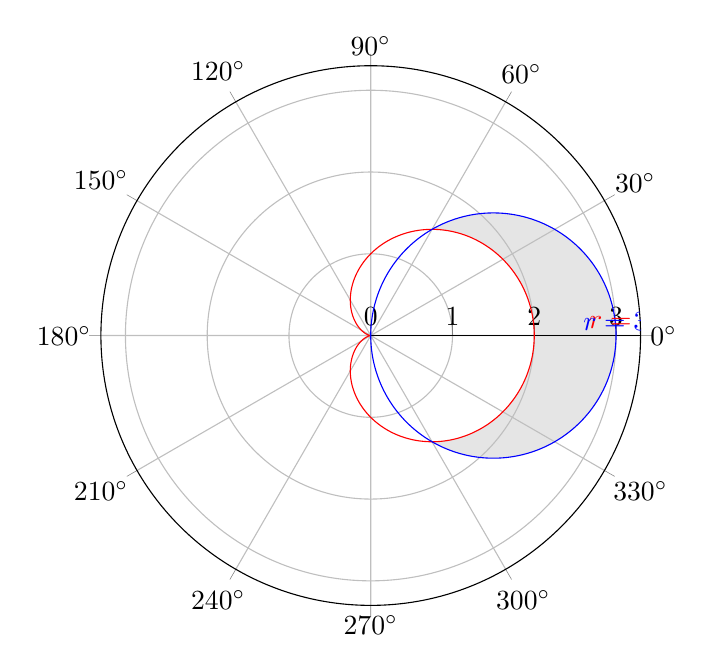
\begin{tikzpicture}
\pgfplotsset{set layers}
  \begin{polaraxis}[xticklabel={$ \pgfmathprintnumber{\tick}^{\circ} $}]
    \addplot[domain=-60:60,samples=500, draw=none, fill=gray!20, on layer=axis background] {3*cos(x)} \closedcycle;
    \addplot[domain=-60:60,samples=500, draw=none, fill=white, on layer=axis background] {1+cos(x)} \closedcycle;
    \addplot[domain=0:360,samples=1000, color=red] {1+cos(x)};
    \addplot[domain=0:360,samples=1000, color=blue] {3*cos(x)};
    \node[red,label kurva,anchor=south west] at (rel axis cs:0.16,0.79) {$r=1+\cos\theta$};
    \node[blue,label kurva,anchor=south west] at (rel axis cs:0.78,0.76) {$r=3\cos\theta$};
    \end{polaraxis}
                \end{tikzpicture}
            \end{center}
            \begin{align*}
L &= 2\int_0^{\pi/3} \frac{1}{2}(3\cos \theta)^2 \, d\theta - 2\int_0^{\pi/3} \frac{1}{2}(1+\cos \theta)^2 \, d\theta\\
&= \int_0^{\pi/3} 9\cos^2 \theta - (1 + 2\cos \theta + \cos^2 \theta) \, d\theta\\
&= \int_0^{\pi/3} 8\cos^2 \theta - 2\cos \theta - 1 \, d\theta\\
&= \int_0^{\pi/3} 8\qty(\frac{1+\cos (2\theta)}{2}) - 2\cos \theta - 1 \, d\theta\\
&= \int_0^{\pi/3} 4 + 4\cos (2\theta) - 2\cos \theta - 1 \, d\theta\\
&= \int_0^{\pi/3} 3 + 4\cos (2\theta) - 2\cos \theta \, d\theta\\
&= \left[3\theta + 2\sin (2\theta) - 2\sin \theta\right]_0^{\pi/3}\\
&= \left(3\cdot \frac{\pi}{3} + 2\cdot \frac{\sqrt{3}}{2} - 2\cdot \frac{\sqrt{3}}{2}\right) - \left(0 + 0 - 0\right)\\
&= \begin{jawaban}{\pi}\end{jawaban}
\end{align*}
                }
            \end{jawab}
            \item Hitunglah luas daerah di luar lingkaran $r=3\cos\theta$ dan di dalam kardioda $r=1+\cos\theta$.\\
            \begin{jawab}
                [luas daerah]{
                Berdasarkan perhitungan dan gambar pada soal sebelumnya, didapatkan bahwa luas daerah tersebut merupakan luas daerah yang dibatasi oleh kardioda $r=1+\cos\theta$ pada interval $\theta$ dari $\pi/3$ hingga $5\pi/3$ dikurangi luas daerah di dalam lingkaran $r=3\cos\theta$ pada interval $\theta$ dari $\pi/3$ hingga $2\pi/3$. Karena kedua kurva tersebut simetris terhadap sumbu $x$, kita dapat menghitung luasnya dengan mengalikan dua kali luas daerah di atas sumbu-$x$, yaitu luas daerah di dalam kardioda $r=1+\cos\theta$ pada interval $\theta$ dari $\pi/3$ hingga $\pi$ dikurangi dengan luas daerah di dalam lingkaran $r=3\cos\theta$ pada interval $\theta$ dari $\pi/3$ hingga $\pi/2$. Didapatkan luasnya adalah
            \begin{center}
                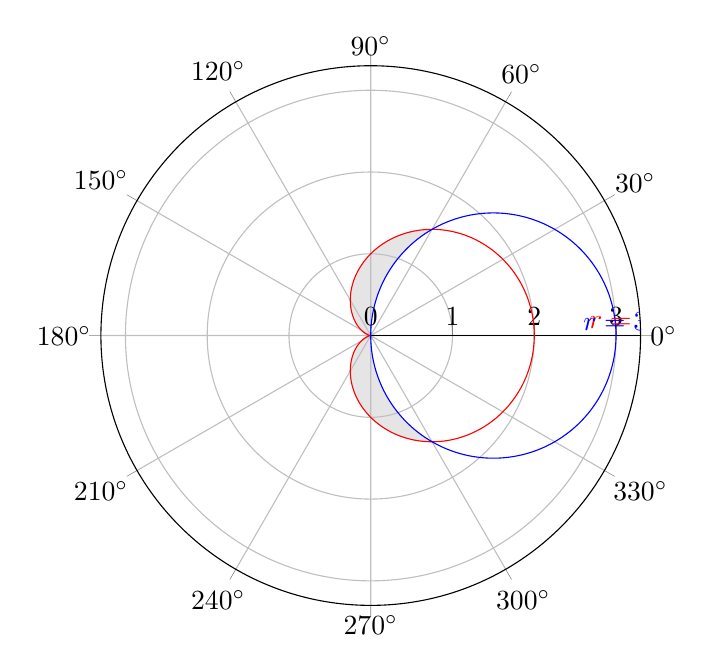
\begin{tikzpicture}
\pgfplotsset{set layers}
  \begin{polaraxis}[xticklabel={$ \pgfmathprintnumber{\tick}^{\circ} $}]
    \addplot[domain=0:360,samples=1000, draw=none, fill=gray!20, on layer=axis background] {1+cos(x)} \closedcycle;
    \addplot[domain=-60:60,samples=500, draw=none, fill=white, on layer=axis background] {1+cos(x)} \closedcycle;
    \addplot[domain=60:90,samples=300, draw=none, fill=white, on layer=axis background] {3*cos(x)} \closedcycle;
    \addplot[domain=-90:-60,samples=300, draw=none, fill=white, on layer=axis background] {3*cos(x)} \closedcycle;
    \addplot[domain=0:360,samples=1000, color=red] {1+cos(x)};
    \addplot[domain=0:360,samples=1000, color=blue] {3*cos(x)};
    \node[red,label kurva,anchor=south west] at (rel axis cs:0.16,0.79) {$r=1+\cos\theta$};
    \node[blue,label kurva,anchor=south west] at (rel axis cs:0.78,0.76) {$r=3\cos\theta$};
    \end{polaraxis}
                \end{tikzpicture}
            \end{center}
                \begin{align*}
L &= 2\int_{\pi/3}^{\pi} \frac{1}{2}(1+\cos \theta)^2 \, d\theta - 2\int_{\pi/3}^{\pi/2} \frac{1}{2}(3\cos \theta)^2 \, d\theta\\
&= \int_{\pi/3}^{\pi} (1 + 2\cos \theta + \cos^2 \theta) \, d\theta - \int_{\pi/3}^{\pi/2} 9\cos^2 \theta \, d\theta\\
&= \int_{\pi/3}^{\pi} \left(1 + 2\cos \theta + \frac{1 + \cos(2\theta)}{2}\right) \, d\theta - \int_{\pi/3}^{\pi/2} \frac{9}{2}(1 + \cos(2\theta)) \,d\theta\\
&= \int_{\pi/3}^{\pi} \left(\frac{3}{2} + 2\cos \theta + \frac{\cos(2\theta)}{2}\right) \, d\theta - \int_{\pi/3}^{\pi/2} \left(\frac{9}{2} + \frac{9}{2}\cos(2\theta)\right) \, d\theta\\
&= \left[\frac{3}{2}\theta + 2\sin \theta + \frac{\sin(2\theta)}{4}\right]_{\pi/3}^{\pi} - \left[\frac{9}{2}\theta + \frac{9}{4}\sin(2\theta)\right]_{\pi/3}^{\pi/2}\\
&= \left(\frac{3\pi}{2} + 0 + 0\right) - \left(\frac{3\pi}{6} + 2\cdot \frac{\sqrt{3}}{2} + \frac{\sin(2\pi/3)}{4}\right) - \left(\frac{9\pi}{4} + 0\right) + \left(\frac{9\pi}{6} + \frac{9}{4}\cdot \frac{\sqrt{3}}{2}\right)\\
&= \frac{3\pi}{2} - \frac{3\pi}{6} - \sqrt{3} - \frac{\sqrt{3}}{8} - \frac{9\pi}{4} + \frac{9\pi}{6} + \frac{9\sqrt{3}}{8}\\
&=\begin{jawaban}{\frac{\pi}{4}}\end{jawaban}
                \end{align*}}
                \end{jawab}
                \item Hitunglah luas daerah yang dibatasi oleh loop dalam dari limacon $r=1+2\cos\theta$.\\
                \begin{jawab}
                [luas daerah]{
                Untuk menghitung luas daerah yang dibatasi oleh loop dalam dari limacon $r=1+2\cos\theta$, perlu menggambar limacon tersebut sebagai berikut:
                Loop dalam terjadi saat nilai $r$ berubah tanda, sehingga batasnya diperoleh dari
                \begin{penting}[]{menyelesaikan $1+2\cos\theta=0$}
                \end{penting}
                sebagai berikut:
            \allowdisplaybreaks
\begin{align*}
1+2\cos\theta=0 \qquad \Longleftrightarrow \qquad \cos\theta=-\frac{1}{2}.
\end{align*}
Jadi, batas loop dalamnya adalah \begin{penting}[]{$\theta=\frac{2\pi}{3}$}\end{penting} dan \begin{penting}[]{$\theta=\frac{4\pi}{3}$}\end{penting}.
            \begin{center}
                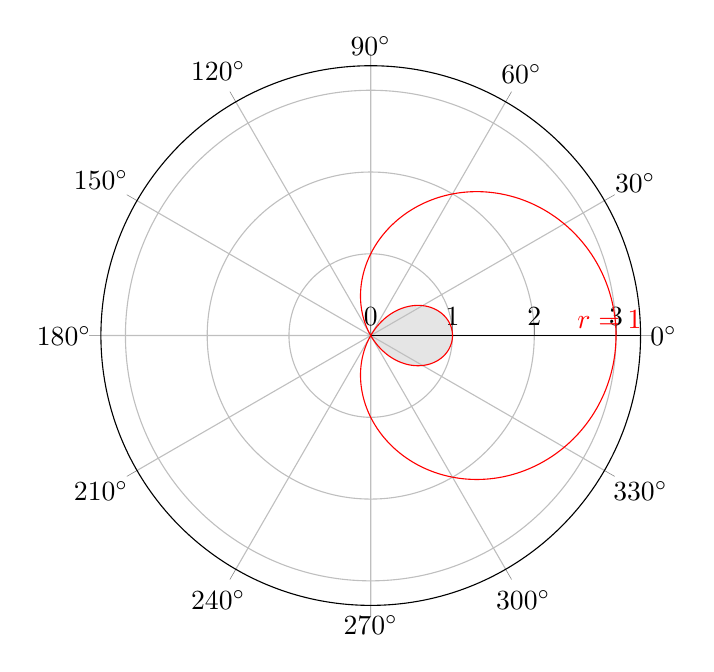
\begin{tikzpicture}
\pgfplotsset{set layers}
  \begin{polaraxis}[xticklabel={$ \pgfmathprintnumber{\tick}^{\circ} $}]
    \addplot[domain=0:360,samples=1000, color=red, save path=\limacon] {1+2*cos(x)};
    \addplot[domain=120:240,samples=400, draw=none, save path=\loopdalam] {1+2*cos(x)};
    \node[red,label kurva,anchor=south west] at (rel axis cs:0.68,0.74) {$r=1+2\cos\theta$};
    \pgfonlayer{axis background}
    \fill[gray!20, reuse path=\loopdalam];
    \endpgfonlayer
    \end{polaraxis}
                \end{tikzpicture}
            \end{center}
            Karena daerah tersebut simetris terhadap sumbu $x$, kita dapat menghitung luasnya dengan mengalikan dua kali luas daerah yang dibatasi oleh kurva tersebut pada interval $\theta$ dari $2\pi/3$ hingga $\pi$. 
            Oleh karena itu, luas daerah yang dibatasi oleh loop dalam dari limacon tersebut dapat dihitung dengan menggunakan rumus luas kurva polar sebagai berikut:   
            \begin{align*}
L &= 2\int_{2\pi/3}^{\pi} \frac{1}{2}(1+2\cos \theta)^2 \, d\theta\\
&= \int_{2\pi/3}^{\pi} (1 + 4\cos \theta + 4\cos^2 \theta) \, d\theta\\
&= \int_{2\pi/3}^{\pi} \left(1 + 4\cos \theta + 4\cdot \frac{1 + \cos(2\theta)}{2}\right) \, d\theta\\
&= \int_{2\pi/3}^{\pi} \left(3 + 4\cos \theta + 2\cos(2\theta)\right) \, d\theta\\
&= \left[3\theta + 4\sin \theta + \sin(2\theta)\right]_{2\pi/3}^{\pi}\\
&= \left(3\pi + 0 + 0\right) - \left(3\cdot \frac{2\pi}{3} + 4\cdot \frac{\sqrt{3}}{2} + \sin\left(\frac{4\pi}{3}\right)\right)\\
&= 3\pi - 2\pi - 2\sqrt{3} + \frac{\sqrt{3}}{2}\\
&= \begin{jawaban}{\pi - \frac{3\sqrt{3}}{2}}\end{jawaban}
                \end{align*}
                 }
                 \end{jawab}
                 \item Dapatkan luas daerah dari irisan kardioida $r=2-2\cos\theta$ dan kardioida $r=2+2\cos\theta$.
                 \begin{jawab}
                [luas daerah]{
                Untuk menghitung luas daerah irisan dari dua kardioida, kita perlu mencari titik potong antara kedua kurva tersebut. Titik potong terjadi ketika $r$ dari kedua kurva sama, yaitu:
\begin{align*}
2 - 2\cos \theta &= 2 + 2\cos \theta\\
-2\cos \theta &= 2\cos \theta\\
-4\cos \theta &= 0\\
\cos \theta &= 0\\
\theta &= \frac{\pi}{2}, \frac{3\pi}{2}
\end{align*}
Jadi, titik potong antara kedua kurva tersebut terjadi pada \begin{penting}[]{$\theta=\frac{\pi}{2}$}\end{penting} dan \begin{penting}[]{$\theta=\frac{3\pi}{2}$}\end{penting}. Berikut adalah gambar dari kedua kurva tersebut:
            \begin{center}
                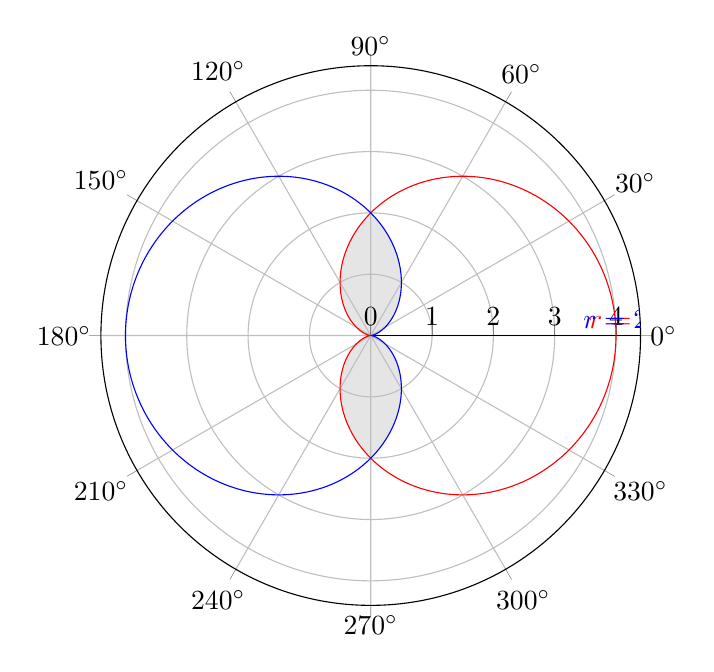
\begin{tikzpicture}
\pgfplotsset{set layers}
  \begin{polaraxis}[xticklabel={$ \pgfmathprintnumber{\tick}^{\circ} $}]
    \addplot[domain=0:90,samples=500, draw=none, fill=gray!20, on layer=axis background] {2-2*cos(x)} \closedcycle;
    \addplot[domain=90:270,samples=500, draw=none, fill=gray!20, on layer=axis background] {2+2*cos(x)} \closedcycle;
    \addplot[domain=270:360,samples=500, draw=none, fill=gray!20, on layer=axis background] {2-2*cos(x)} \closedcycle;
    \addplot[domain=0:360,samples=1000, color=red] {2+2*cos(x)};
    \addplot[domain=0:360,samples=1000, color=blue] {2-2*cos(x)};
    \node[red,label kurva,anchor=south west] at (rel axis cs:0.16,0.79) {$r=2+2\cos\theta$};
    \node[blue,label kurva,anchor=south west] at (rel axis cs:0.78,0.76) {$r=2-2\cos\theta$};
    \end{polaraxis}
                \end{tikzpicture}
            \end{center}
            Karena kedua kurva tersebut simetris terhadap sumbu $x$, kita dapat menghitung luasnya dengan mengalikan dua kali luas daerah di atas sumbu-$x$, yaitu pada interval $\theta$ dari $\pi/2$ hingga $3\pi/2$. 
            Luas daerah tersebut adalah luas daerah di dalam kardioida $r=2+2\cos\theta$ pada interval $\theta$ dari $\pi/2$ hingga $3\pi/2$ dikurangi dengan luas daerah di dalam kardioida $r=2-2\cos\theta$ pada interval $\theta$ dari $\pi/2$ hingga $3\pi/2$. Didapatkan luasnya adalah 
            \begin{align*}L &= 2\int_{\pi/2}^{3\pi/2} \frac{1}{2}(2+2\cos \theta)^2 \, d\theta - 2\int_{\pi/2}^{3\pi/2} \frac{1}{2}(2-2\cos \theta)^2 \, d\theta\\
&=  2\int_{\pi/2}^{3\pi/2} \frac{1}{2}4(1+\cos \theta)^2 \, d\theta - 2\int_{\pi/2}^{3\pi/2} \frac{1}{2}4(1-\cos \theta)^2 \, d\theta\\
&= 4\int_{\pi/2}^{3\pi/2} (1 + 2\cos \theta + \cos^2 \theta) \, d\theta - 4\int_{\pi/2}^{3\pi/2} (1 - 2\cos \theta + \cos^2 \theta) \, d\theta\\
&= 4\int_{\pi/2}^{3\pi/2} \left(1 + 2\cos \theta + \frac{1 + \cos(2\theta)}{2}\right) \, d\theta - 4\int_{\pi/2}^{3\pi/2} \left(1 - 2\cos \theta +  \frac{1 + \cos(2\theta)}{2}\right) \, d\theta\\
&= 4\int_{\pi/2}^{3\pi/2} \left(\frac{3}{2} + 2\cos \theta + \frac{\cos(2\theta)}{2}\right) \, d\theta - 4\int_{\pi/2}^{3\pi/2} \left(\frac{3}{2} - 2\cos \theta + \frac{\cos(2\theta)}{2}\right) \, d\theta\\
&= 4\left[\frac{3}{2}\theta + 2\sin \theta + \frac{\sin(2\theta)}{4}\right]_{\pi/2}^{3\pi/2} - 4\left[\frac{3}{2}\theta - 2\sin \theta + \frac{\sin(2\theta)}{4}\right]_{\pi/2}^{3\pi/2}\\
&= 4\left(\frac{9\pi}{4} + 0 + 0\right) - 4\left(\frac{9\pi}{4} + 0 + 0\right)\\
&= \begin{jawaban}{0}\end{jawaban}
\end{align*}
                 }
                 \end{jawab}
            \end{enumerate}
\end{document}
